\documentclass[../../main.tex]{subfiles}

\begin{document}

\section{Linters}
\textbf{Linting} is the process of analysing source code to identify and report issues related to coding style and potential logical errors.
The term originates from the \texttt{lint} program~\cite{johnson_lint_1978}, which examined C source code for bugs, as well as wasteful code patterns that may be legal but error-prone.
The tool was also utilised to enforce portability restrictions which aided users in writing portable code that could be compiled on multiple platforms.
Since the release of \texttt{lint}, many linting tools, known as \textbf{linters}, have been developed for a wide range of programming languages.

Nowadays, many linters can be integrated into \textsc{ide}s, where code analysis performed by the linter is run incrementally in the background.
Any violations found by the linter are displayed directly in the editor as warnings or errors at the relevant locations in the source code.
This brings early, real-time feedback to the programmer, allowing them to address issues as they write code, with minimal interruption to their development workflow.
Linters can also be integrated as part of the code review process, or into continuous integration (\textsc{ci}) pipelines to ensure that code adheres to a set of standards before being merged into the main codebase.

Although the traditional definition for linting is concerned only with \emph{detecting} issues in code, modern linters have broadened their scope significantly.
In addition to detecting issues, many linters provide \emph{auto-fix} capabilities to correct issues by automatically rewriting the offending code snippets.
This feature is often integrated into \textsc{ide}s as well: the popular Language Server Protocol for defining \textsc{ide} features enables these auto-fix features via \emph{code actions}~\cite{gunasinghe_lsp_2022}.
When a section of code is highlighted by a linter warning, a user can apply a code action to automatically fix the issue with a single click.

% Linters and related static analysis tools are increasingly becoming more important in modern software development, as modern code continues to become more complex and difficult to reason about.
% Industry leaders, such as Google~\cite{sadowski_analysis-google_2018} and Meta/Facebook~\cite{calcagno_moving-facebook_2015}, have embraced these tools as integral components of their software development workflows.
% The use of automated tools to detect potential issues is not only faster but in some cases more effective than human review, saving developer time and reducing error rates in the development process.

\subsection{Categories of Lint Rules}

Many linters are configurable with a set of \emph{rules}, which specify the categories of issues that the linter should detect.
These rules can be enabled or disabled by users, allowing them to customise the linter to their needs.
Rules are usually grouped by purpose: some rules are concerned with simply improving code style, while others are concerned with detecting suspicious code patterns indicative of potential bugs.

\subsubsection{Style checks and code quality}
Linters can suggest opportunities to improve code by utilising language features in a more idiomatic manner.
Snippets of code that violate these stylistic rules are not necessarily incorrect, but should be fixed as they may be harder to read or maintain in the long term.
Furthermore, many idiomatic practices exist to avoid common pitfalls that could lead to unintended behaviour.
By highlighting good practices, linters can help users avoid these common mistakes that may cause bugs.
For example, \emph{ESLint}\footnote{\url{https://eslint.org/docs/latest/rules/}}, one of the most popular JavaScript linters, warns against common JavaScript pitfalls such as using the regular equality operator \texttt{==} instead of its type-safe alternative \texttt{===}.

A well-designed linter can help programmers learn about useful language constructs by suggesting them in the context of their code, aiding them in adhering to best practices and common style conventions.
This category of rules is therefore especially helpful as an educational tool for new users of a language, who may be unaware of these idioms.
For example, the \emph{Clippy}\footnote{\url{https://doc.rust-lang.org/clippy/}} linter for Rust~\cite{li_clippy_2023} categorises a collection of rules as \texttt{clippy::complexity} rules to detect code that does something simple in a complex way and suggests a simpler alternative.
\Cref{fig:hlint-example} provides an example of a similar rule in Haskell, from the \textit{HLint}\footnote{\url{https://hackage.haskell.org/package/hlint}} linter.
The rule suggests to rewrite the function into an equivalent but more concise form via $\eta$-reduction, presented to the user as a code action that can be applied automatically.

\begin{figure}[htbp]
  \vspace{3ex}
  \centering
  \begin{subfigure}{0.45\textwidth}
    \centering
    \begin{minted}[frame=single]{haskell}
      foo xs = map (+1) xs
    \end{minted}
    \caption{A Haskell function \texttt{foo}, which can be made more concise using $\eta$-reduction.}
  \end{subfigure}
  \hfill
  \begin{subfigure}{0.45\textwidth}
    \centering
    \begin{minted}[frame=single,escapeinside=||]{text}
      Eta reduce
      Found:
        foo xs = map (+ 1) xs
      Why not:
        foo = map (+ 1)
      |\textcolor{gray}{hlint(refact:Eta reduce)}|
    \end{minted}
    \caption{The linter warning shown for \texttt{foo}.}
  \end{subfigure}
  \caption{An example of a warning from the Haskell linter \texttt{hlint}, suggesting a fix that a user can choose to automatically apply.}
  \label{fig:hlint-example}
\end{figure}

\paragraph{Domain-specific idioms}
A library or especially an embedded \textsc{dsl} may require a particular style of usage that is different from the host language~\cite{hora_domain_2012}.
The majority of linters are designed for general-purpose application domains, so they are unlikely to detect issues specific to a more specialised domain.
Therefore, linters may be developed for specific libraries or \textsc{dsl}s, with their own set of domain-specific rules.
In this case, the accompanying linter can benefit users and improve developer productivity in a similar manner to general-purpose linters: common misuses can be detected and sometimes automatically fixed, and users can be directed to relevant documentation to learn more about correct usage.
For instance, the \emph{xUnit.net} testing framework for C\# is accompanied by the \texttt{xunit.analyzers}\footnote{\url{https://github.com/xunit/xunit.analyzers}} package which provides linting rules to enforce best practices specific to \emph{xUnit}.

\subsubsection{Code smells and opportunities for refactoring}
Code refactoring is a well-established practice in software development.
In his influential book \emph{Refactoring: Improving the Design of Existing Code}~\cite{fowler_refactoring_2018}, Fowler defines \textbf{refactoring} as ``the process of changing a software system in such a way that it does not alter the external behaviour of the code yet improves its internal structure''.
Refactoring may be employed to eliminate \textbf{code smells}, which are surface indications that could indicate deeper problems in the system.
Code smells are not necessarily problematic on their own, however, they may lead to issues such as bugs or poor maintainability if left unchecked.
They are conceptually similar to the stylistic issues mentioned earlier, however they may encompass higher-level structural and design-based problems that are not easily fixed by simple stylistic changes.
Examples of code smells include duplicated code, which can be hard to update without introducing bugs, and long methods, which can be difficult to understand and maintain.
Therefore, it is often productive to refactor code to eliminate code smells, even if the code is still correct and functional.

Certain linting rules can aid in the refactoring process by broadly identifying code smells and candidate areas for refactoring, suggesting appropriate actions that the user can take.
As an example, a linter may detect a fragment of code that is repeated in multiple places: this is a code smell, as discussed previously.
The linter may then suggest a code action to automatically apply an \emph{Extract Method}~\cite{fowler_refactoring_2018} refactoring to avoid code duplication: \cref{fig:extract-function-intellij} demonstrates how this automatic refactoring process can be performed in the IntelliJ IDEA\footnote{\url{https://www.jetbrains.com/idea/}} \textsc{ide}.

\begin{figure}[htbp]
  \centering
  \begin{subfigure}{\textwidth}
    \centering
    \begin{minted}[frame=single,highlightlines={4-5},linenos]{scala}
      object Main {
        def main(args: Array[String]): Unit = {
          val bankDetails = getBankDetails()
          println(s"Account name: ${bankDetails.name}")
          println(s"Account balance: ${bankDetails.balance}")
        }
      }
    \end{minted}
    \caption{A snippet of Scala code. A user may wish to extract the highlighted lines into a separate function.}
    \label{fig:extract-function-intellij-before}
  \end{subfigure}
  \begin{subfigure}{\textwidth}
    \centering
    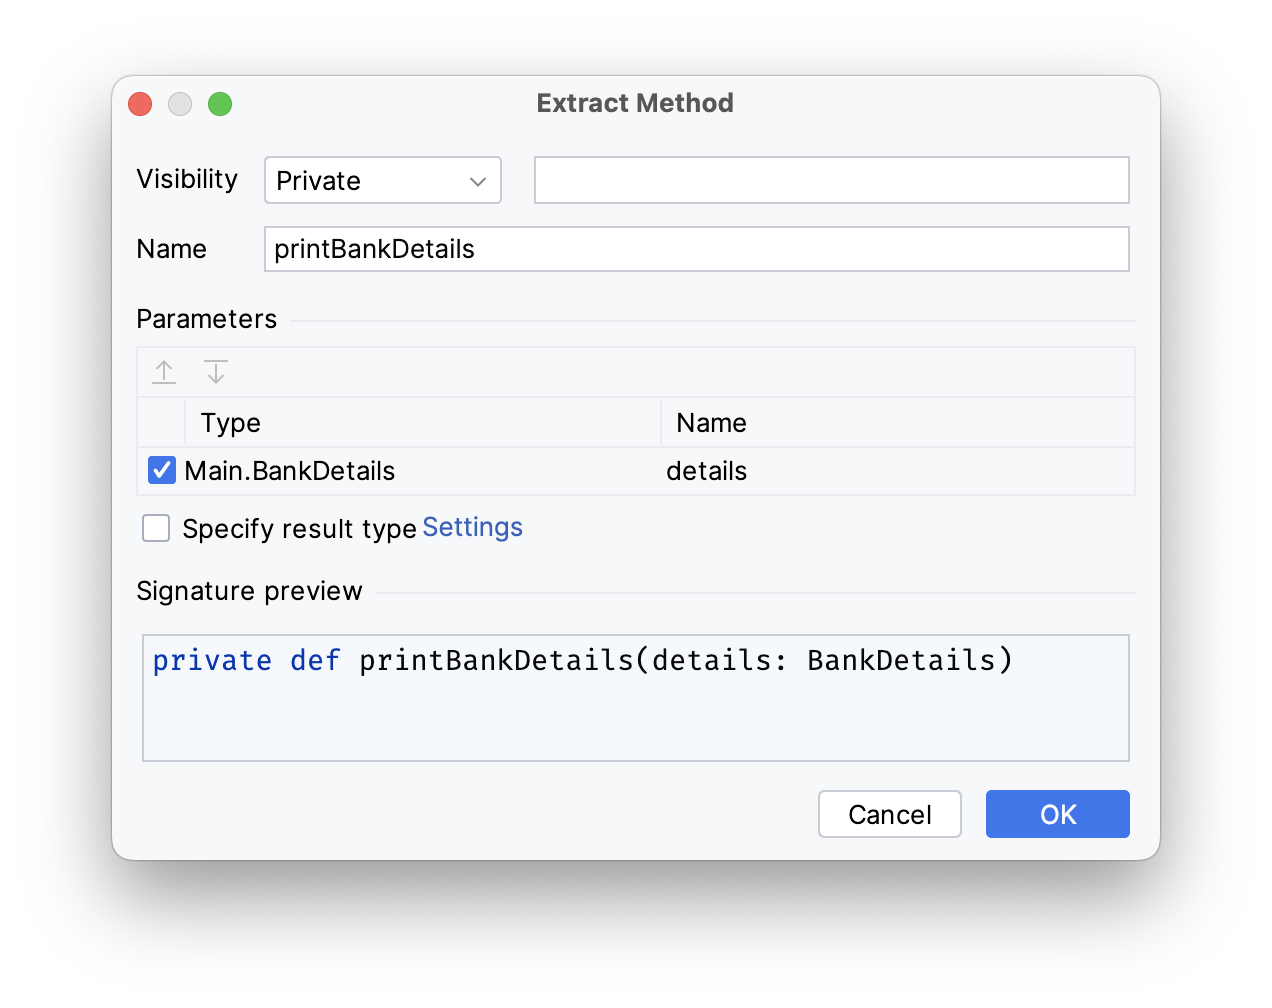
\includegraphics[width=0.75\textwidth]{src/background/extract-function-intellij.png}
    \caption{When a user selects the highlighted lines from \cref{fig:extract-function-intellij-before} in IntelliJ IDEA, choosing the \emph{Extract Method} refactoring will open this dialogue to preview changes before applying them.}
    \label{fig:extract-function-intellij-dialogue}
  \end{subfigure}
  \begin{subfigure}{\textwidth}
    \vspace{3ex} % TODO: ew
    \centering
    \begin{minted}[frame=single,highlightlines={4,7-10},linenos]{scala}
      object Main {
        def main(args: Array[String]): Unit = {
          val bankDetails = getBankDetails()
          printBankDetails(bankDetails)
        }

        private def printBankDetails(details: BankDetails): Unit = {
          println(s"Account name: ${details.name}")
          println(s"Account balance: ${details.balance}")
        }
      }
    \end{minted}
    \caption{The result of applying the \emph{Extract Method} refactoring using the chosen parameters in \cref{fig:extract-function-intellij-dialogue}.}
  \end{subfigure}
  \caption{An example of the \emph{Extract Method} refactoring in IntelliJ IDEA.}
  \label{fig:extract-function-intellij}
\end{figure}

\subsubsection{Likely bugs or errors}
In some cases, linters may be able to detect with relatively high confidence that a piece of code is likely to contain a bug.
Rules that detect more egregious issues like this are helpful for even experienced users to avoid common pitfalls.
For example, \emph{Clippy} has \texttt{clippy::correctness} rules which identify code very likely to be incorrect or useless, and \texttt{clippy::suspicious} rules for code that is \emph{very sus} but could be a false positive.
\emph{ESLint} also provides several rules to warn against code patterns that are likely to cause runtime errors, such as re-assigning a \texttt{const} variable.

Again, linters may attempt to provide code fixes for these issues where possible.
However, these issues are usually more complex, which may limit the effectiveness or usefulness of auto-fixes: in the case of a suspicious code pattern, the programmer's intent may not be clear, causing the linter to suggest a fix that does not align with the user's expectations.

\subsection{Implementing Linters}
\subsubsection{Static vs Dynamic Analysis}
\emph{Static analysis} analyses source code to extract information about its behaviour without executing the program itself.
% Static analysis tools can perform a variety of tasks, ranging from detecting possible bugs~\cite{johnson_lint_1978,hovemeyer_finding-bugs_2004} to formal software verification of program properties~\cite{blanchet_static-analyzer_2003}.
This is in contrast to \emph{dynamic analysis}, which is performed on programs as they run to observe their actual runtime behaviour.
Both techniques have their own advantages and disadvantages, and the choice between them depends on the desired properties of a tool.
Dynamic analysers are \emph{precise} in that they only observe what a program can actually do, but requires a whole system that can be executed.
On the other hand, static analysers can be more lightweight and can be applied to incomplete systems, since they do not require the program to be run.
However, the trade-off is that static analysis is generally more \emph{imprecise} since it must approximate the possible behaviours of the program.

Linters should be fast and lightweight, as it is desirable for them to provide feedback to the user in real-time within the \textsc{ide}.
Furthermore, it is desirable for them to be able to provide warnings on incomplete programs and analyse even just fragments of code for suspicious code patterns.
For these reasons, the vast majority of linters are static analysis tools.

% TODO: might be worth talking about soundness and completeness
% https://stackoverflow.com/questions/12884623/static-and-dynamic-code-analysis
% Most practical static checkers for JavaScript [3, 2, 1, 4] and other languages [29, 11] take a pragmatic view and favor a relatively low false positive rate over soundness

% In some instances, however, dynamic languages such as JavaScript present challenges for static analysis due to their dynamic runtime nature.
% This has led to the exploration of linters that incorporate dynamic analysis techniques to identify issues that static methods cannot detect~\cite{gong_dlint_2015}.
% Despite these developments, state-of-the-art JavaScript linters utilised in industry, such as \emph{ESLint}, still solely rely on static analysis.
% Regardless, since Scala is strongly and statically-typed it does not suffer from the same downsides, so the focus of this thesis will be on implementing \texttt{parsley-garnish} using static analysis.

% TODO: discussion of parsley-debug's dynamic analysis capabilities (should this go here?)

\subsubsection{Metaprogramming}
Linters that provide code fixes are \emph{metaprograms}: they are programs that manipulate programs.
Auto-fixes and refactorings are performed as source-to-source transformations, which may be implemented as simple text-based replacements or more robust rewrite rules that operate on the abstract syntax tree (\textsc{ast}) of the source code.

Analyses over \textsc{ast}s are typically semantic-aware, respecting scoping rules and type information to provide more accurate code fixes.
This semantic information is often provided by the compiler -- some linters opt to run during compilation as a compiler plugin, while others run as a separate tool after compilation.
Lint-on-compile and lint-after-compile tools both have their own advantages and disadvantages, and the choice between them depends on the use case~\cite{sadowski_analysis-google_2018}.

\subsubsection{Code-Fixing Approaches}
% Partial verificationtechniques have been proposed. These techniques prove thatsome desired property of a program holds for all possible ex-ecutions.  Such techniques may be complete or incomplete;if incomplete, then the analysis may be unable to prove thatthe desired property holds for some correct programs.  Fi-nally,unsoundtechniques can identify “probable” bugs, butmay miss some real bugs and also may emit some inaccuratewarnings.

\TODO{
  Our approach is formal methods using domain-specific knowledge of parser laws
  Not data-driven or ML/LLM approach
}


\section{Writing Linters for Scala}

\TODO{
  DSL linting is hard but luckily Parsley is an eDSL so we can just use Scala metaprogramming utilities
}

\subsection{Choice of Tooling}
The goal of \texttt{parsley-garnish} is to provide linting and refactoring capabilities for the \texttt{parsley} parser combinator library.
Since \texttt{parsley} is a Scala library, this project must be implemented using a tool capable of statically analysing Scala code.
This section will therefore discuss and evaluate the choices available for implementing \texttt{parsley-garnish}.

\paragraph{Scala compiler plugins}
The most powerful approach would be to implement \texttt{parsley-garnish} as a compiler plugin~\cite{pickering_plugins_2019}.
Using the low-level compiler \textsc{api}, it is possible to perform arbitrary code transformations at any step of the compilation process.
Compiler plugins therefore offer full freedom to extend the Scala compiler with extra functionality, such as extra passes for code analysis and emitting lint warnings as diagnostics or even compiler errors.

However, this approach has several drawbacks.
Firstly, compiler plugins are tightly coupled with the compiler itself, and therefore not portable across major compiler versions.
% https://github.com/mattmoore/scala-compiler-plugins is a good reference, in case I need to revisit this
For instance, plugins written for the Scala 3 compiler, known as \texttt{dotty}, are completely incompatible with Scala 2 plugins~\cite{lampepfl_changes_2022}.
Additionally, developing compiler plugins requires a deep understanding of arcane and poorly documented compiler internals.
Exposing the full compiler \textsc{api} permits unsafe operations that may violate undocumented invariants assumed by the compiler, leading to exceptions during compilation or even malformed bytecode~\cite{sherwany_refactoring_2015}.
The lack of higher-level abstractions also makes it difficult to implement even trivial tasks such as renaming a field.

For these reasons, it would be preferable to explore other tools that may use compiler plugins themselves but provide a higher-level interface for implementing code analysis and transformations.

\paragraph{Scalameta}
\textit{Scalameta}\footnote{\url{https://scalameta.org/}} is a metaprogramming framework for Scala that provides a unified interface for performing common metaprogramming tasks.
Many Scala tools are built with Scalameta, most notably the \emph{Metals}\footnote{\url{https://scalameta.org/metals/}} \textsc{lsp} server for Scala.
It provides a high-level syntactic \textsc{api} for transforming and pretty-printing Scala source code, as well as a semantic \textsc{api} providing access to semantic information such as type inference and name resolution.
Scalameta builds upon the earlier \texttt{scala.reflect} metaprogramming framework, unifying runtime and compile-time metaprogramming under a single \textsc{api}.
Previously under \texttt{scala.reflect}, source code was parsed into lossy trees that discarded syntactic \emph{trivia} such as comments and whitespace~\cite{burmako_scalameta_2017}.
On the other hand, Scalameta trees are fully lossless and preserve all syntactic details: a crucial feature for code transformations and refactorings that must preserve formatting details.

Scalameta's semantic \textsc{api} is powered by \textit{SemanticDB}, a compiler-agnostic data model for semantic information in Scala programs.
This allows Scalameta to extract semantic information via compiler plugins that emit data in the SemanticDB format.
Thus, Scalameta can work with any compiler that supports SemanticDB, rather than being tied to a specific compiler implementation.

Since Scalameta provides a high-level interface for manipulating syntactic and semantic information, it is a promising choice for this project.
Being able to access semantic information is especially helpful for implementing more complex code analyses.
However, Scalameta's primary focus is on providing a general metaprogramming framework and therefore lacks \textsc{api} support specifically for implementing linting and refactoring rules.
For example, the Scalameta tree transformation utilities do not fully preserve formatting details when pretty-printed, despite the underlying trees containing this information.

\paragraph{Scalafix}
\textit{Scalafix}\footnote{\url{https://scalacenter.github.io/scalafix/}} is a code linting and rewriting tool built on top of Scalameta.
It provides a higher-level \textsc{api} over Scalameta's tree transformation capabilities, specifically designed for implementing fine-grained code transformations that preserve the original formatting of the source file.
Scalafix provides a framework for implementing linting rules to emit diagnostic warnings, as well as rewrite rules to perform automated code transformations~\cite{geirsson_catch_2017}.
Since it is built on Scalameta, a major advantage of Scalafix is that it is also compiler-agnostic and could be integrated into any \textsc{ide} if a plugin is developed for it.

Originally, Scalafix was designed to help automate the process of migrating code from Scala 2 to 3, which involved many breaking changes to the language~\cite{geirsson_scalafix_2016}.
However, Scalafix has since evolved into a general-purpose tool for implementing generic code transformations and analyses.
Scalafix rules can be either \emph{syntactic} or \emph{semantic} depending on whether they require semantic information, such as type signatures, to perform their analysis~\cite{scalacenter_scalafix_2024}.
Syntactic rules are faster to run, operating purely on the \textsc{ast} without needing to invoke compilation, but are more limited in the analyses they can perform.
Semantic rules, on the other hand, are more complicated to run: they require augmenting the Scala compiler with the SemanticDB compiler plugin to provide Scalafix with the required semantic information.
They are also slower as a result, since they require the source file to be compiled.

% Scalafix is growing to become the de-facto modern successor to earlier refactoring tools such as Abide\footnote{\url{https://contributors.scala-lang.org/t/whats-the-status-of-abide/}} and \texttt{scala-refactoring}\footnote{\url{https://github.com/scala-ide/scala-refactoring}}.
% \texttt{scala-refactoring} used \texttt{scala.reflect} to implement code transformations, with much extra work utilising the Scala Presentation Compiler \textsc{ast} to preserve formatting details lost by \texttt{scala.reflect}.
% As a result, maintaining the library became difficult and the project was abandoned in favour of a clean implementation using Scalameta, which was designed in part to address the shortcomings of \texttt{scala.reflect}.

A drawback of Scalafix is that it is primarily a command-line tool, and currently does not provide an interactive interface within any code editor.
Ideally, users should be able to see inline diagnostics, as well as preview and select auto-fixes interactively like in \cref{fig:extract-function-intellij}.
A Metals integration would be the most favourable outcome, as they already share a Scalameta backend, and it would allow Scalafix to be integrated into any code editor supporting the \textsc{lsp} protocol.
However, at the time of writing, Scalafix only has basic integrations with Metals to run rules, but no interactive in-editor integrations~\cite{jaglin_scalafix_2024}.
This feature request is an open issue on GitHub\footnote{\url{https://github.com/scalameta/metals-feature-requests/issues/230}}, but no timeline has been provided for its implementation.

Nonetheless, Scalafix emerges as the most favourable choice for implementing \texttt{parsley-garnish}.
It provides high-level \textsc{api}s specifically for implementing linting and rewrite rules without necessitating extensive knowledge of compiler internals.
Scalafix is also being actively maintained, with good basic documentation and a growing number of examples of usage in the wild.

\paragraph{Other tools considered}
The main alternate contender to Scalafix is the IntelliJ Scala Plugin\footnote{\url{https://github.com/JetBrains/intellij-scala}}.
However, while the plugin offers superior interactive usage within the IntelliJ IDEA \textsc{ide}, it is tied to the IntelliJ Scala compiler and therefore not portable across other compilers.
To maintain flexibility and not tie \texttt{parsley-garnish} to a particular compiler or code editor, Scalafix is a preferable option.
Furthermore, documentation is less clear on how to write a Scala plugin for IntelliJ compared to the Scalafix documentation.

WartRemover\footnote{\url{https://www.wartremover.org/}} is a linter implemented as a compiler plugin, with support for writing custom rules.
However, it only can emit diagnostics and does not support code fixes, making it unsuitable for \texttt{parsley-garnish}'s goals.

ScalaStyle\footnote{\url{http://www.scalastyle.org/}} is primarily a style checker which also supports custom rules.
However, it is only able to perform syntactic analyses and does not have access to semantic information, restricting the types of analyses it can perform.

% TODO: comparison with clippy (https://doc.rust-lang.org/clippy/development/lint_passes.html) and/or roslyn (https://learn.microsoft.com/en-us/dotnet/csharp/roslyn-sdk/; https://learning.oreilly.com/library/view/roslyn-cookbook/9781787286832/) ?

\subsection{A Crash Course on Scalafix}\label{sec:scalafix}
This \namecref{sec:scalafix} briefly explains how Scalafix rules are written,
providing the Scalafix-specific terminology needed to understand the implementation details of \texttt{parsley-garnish}.

\subsubsection{Rules}
Scalafix rules are implemented as generic top-to-bottom traversals through the Scala \textsc{ast}, represented as a Scalameta \scala{Tree} data structure.
This is achieved with a collection-like \textsc{api}, exposing these operations in the style of standard Scala collection methods such as \scala{traverse} and \scala{collect}.
During traversal, side effects are generated using the \scala{Patch} data structure, which represents either a lint diagnostic or a code rewrite.
Rules are applied file-by-file, and the patches generated by each rule are collected and applied by Scalafix as a batch rewrite after all rules have finished running.

\Cref{fig:syntactic-rule-ex} showcases the basic structure of a simple syntactic rule:
\begin{itemize}
  \item \scala{doc.tree.collect} performs the tree traversal, where \textsc{ast} nodes of interest can be visited via pattern matching.
  \item \scala{case v: Defn.Val if !v.mods.exists(_.is[Mod.Lazy])} visits a \scala{val} definition node that is not already marked as \scala{lazy}.
  \item \scala{Patch.addLeft(v, "lazy ")} describes a patch to add the \scala{lazy} modifier to the left side of the node that was matched on.
\end{itemize}

\begin{figure}[htbp]
\begin{minted}{scala}
class MakeValsLazy extends SyntacticRule("MakeValsLazy") {
  override def fix(implicit doc: SyntacticDocument): Patch = {
    doc.tree.collect {
      case v: Defn.Val if !v.mods.exists(_.is[Mod.Lazy]) => Patch.addLeft(v, "lazy ")
    }.asPatch
  }
}
\end{minted}
\caption{A syntactic rule that makes all \texttt{val} definitions lazy.}
\label{fig:syntactic-rule-ex}
\end{figure}

\subsubsection{Safer Patches Using Quasiquotes}
A careful reader may notice from \cref{fig:syntactic-rule-ex} that the \scala{Patch} rewrite method receives a raw string value, which seems unsafe and could potentially lead to malformed code.
That careful reader would indeed be correct:
Scalafix provides no guarantees that the output of a patch is a well-formed program, and it is the rule author's responsibility to ensure so.

The approach taken by \texttt{parsley-garnish} is to represent intended rewrites as Scalameta \scala{Tree} objects, and only convert them to strings immediately before applying the patch.
\Cref{fig:quasiquote-ex} shows how \emph{quasiquotes}~\cite{shabalin_quasiquotes_2013} can be used as syntactic sugar to construct trees in a convenient manner:
\begin{itemize}
  \item \scala{q"..."} is the quasiquote's string interpolation syntax to build a \scala{Term} node, which is a subclass of \scala{Tree}.
  \item \scala{${...}} is the \emph{splice} or \emph{unquote} operation to insert a term into the constructed tree. Ordinarily, spliced values need to be an instance of a \scala{Tree}, but simple values such as integers (in this case) can be automatically lifted into the appropriate tree node.
  \item \scala{Tree.structure} represents the resulting \scala{Tree} data structure as a string, useful for debugging.
  \item \scala{Tree.syntax} pretty-prints the tree back into its source code representation, which can then be fed into a \scala{Patch}.
\end{itemize}
Quasiquotes expand at compile-time into \scala{Tree} constructors, so they do not preserve formatting details.
This turns out to be very convenient for pretty-printing purposes: often, spliced values may contain superfluous parentheses, which are automatically removed (as seen in the final example within \cref{fig:quasiquote-ex}).

\begin{figure}[htbp]
\begin{minted}{scala}
val x = 1
val tree = q"$x + 2"

println(tree.structure)
// Term.ApplyInfix(
//   Lit.Int(1),
//   Term.Name("+"),
//   Type.ArgClause(Nil),
//   Term.ArgClause(List(Lit.Int(2)), None)
// )

println(tree.syntax)
// 1 + 2
println(q"($tree)".syntax)
// 1 + 2
\end{minted}
\caption{Using Scalameta quasiquotes to construct a tree.}
\label{fig:quasiquote-ex}
\end{figure}

By using quasiquotes instead of raw strings, the syntactic correctness of a rewrite is guaranteed.
However, this safety is not foolproof: quasiquotes are not guaranteed to be well-typed or well-scoped, so the rewritten program still might not be able to compile.
They are also not \emph{hygienic}: generated code will not be able to avoid name clashes with regular code~\cite{burmako_scalameta_2017}.
The lack of hygiene can cause issues with variable capture, allowing a variable to be unintentionally shadowed by a generated variable.
Again, it is the rule author's responsibility to ensure that variable capture does not occur: \cref{sec:function-representation} in part discusses how this is handled in \texttt{parsley-garnish}.

\subsubsection{Semantic Information}
Semantic rules are implemented in the same manner as \cref{fig:syntactic-rule-ex}, but instead take the more powerful \scala{SemanticDocument} as an implicit parameter.
This allows rule authors to query \textsc{ast} nodes for their associated symbols: textual identifiers that represent definitions in the Scala program.
Although symbols are not guaranteed to be unique outside the document they are defined in~\cite{scalameta_semanticdb_spec_2023}, within the context of Scalafix rule authoring, they can be treated as unique since rules are applied per-file.

The following methods are the most important for querying the semantic information associated with a tree node:
\begin{itemize}
  \item \scala{Tree.symbol} retrieves the symbol associated with a node.
  \item \scala{Symbol.info} queries a symbol for any \scala{SymbolInformation} attached to it, including metadata such as its type signature.
  \item \scala{Tree.synthetics} reveals extra compiler-generated tree nodes not present in the original source code, such as implicit conversions or inferred \scala{.apply} methods.
\end{itemize}

Additionally, the \scala{SymbolMatcher} trait provides a convenient way to create predicates that match specific symbols.
\Cref{fig:semantic-rule-ex} demonstrates how symbol matching can be used to detect integer addition operations, emitting a diagnostic warning when found.
The \scala{intAdd} symbol matcher only matches the \scala{+} method on integers, so the rule does not emit a diagnostic for addition operations on other types, as seen in \cref{fig:semantic-rule-ex-example}.

% TODO: Comparison with HLint? https://ndmitchell.com/downloads/slides-static_analysis_of_haskell-11_jul_2017.pdf

\begin{figure}[htbp]
\begin{subfigure}{\textwidth}
\begin{minted}{scala}
class IdentifyIntAddition extends SemanticRule("IdentifyIntAddition") {
  val intAdd = SymbolMatcher.normalized("scala.Int.`+`")

  override def fix(implicit doc: SemanticDocument): Patch = doc.tree.collect {
    case Term.ApplyInfix(_, intAdd(node), _, _) =>
      Patch.lint(IntAdditionLint(node))
  }.asPatch
}

case class IntAdditionLint(tree: Tree) extends Diagnostic {
  override def position: Position = tree.pos
  override def severity: LintSeverity = LintSeverity.Info
  override def message: String = "Found an addition operation on integers"
}
\end{minted}
\caption{A semantic rule that generates lint diagnostics \emph{only} on integer addition operations.}
\label{fig:semantic-rule-ex-impl}
\end{subfigure}
%
\begin{subfigure}{\textwidth}
\vspace{3ex} % TODO: ew
\begin{minted}{scala}
object Main {
  val stringAdd = "parsley" + "garnish"
  val intAdd = 1 + 2
  val floatAdd = 1.0 + 2.0
}

// Main.scala:3:18: info: [IdentifyIntAddition]:
// Found an addition operation on integers
//   val intAdd = 1 + 2
//                  ^
\end{minted}
\caption{An example program showcasing the rule in \cref{fig:semantic-rule-ex-impl}.}
\label{fig:semantic-rule-ex-example}
\end{subfigure}
\caption{An example showing how semantic rules are semantic-aware on overloaded method names.}
\label{fig:semantic-rule-ex}
\end{figure}

% The compiler information that semantic rules use is provided by the \texttt{semanticdb-scalac} compiler plugin.
% This is injected immediately after the \texttt{typer} phase of the \texttt{scalac} Scala compiler, allowing it to harvest and dump semantic information in SemanticDB format.~\cite{scalameta_semanticdb_guide_2023}
% Basically a stripped-down version of \textsc{tast}y (Typed Abstract Syntax Trees)\footnote{\url{https://docs.scala-lang.org/scala3/guides/tasty-overview.html}} but for both scala 2 and 3.
% Scalafix then presents a seamless API to implement semantic rules, allowing users to inspect an AST node and any semantic information associated with it.

\end{document}
